\documentclass{article}
\renewcommand\refname{Referencias}
\renewcommand\contentsname{\'Indice de Conten\'ido}
\usepackage{graphicx}
\graphicspath{{IMG/}}
\usepackage{caption}
\usepackage{subcaption}
\usepackage{float}
\usepackage{listings}
\lstset{
 showstringspaces=false,
 tabsize=2,
 frame=single,
 numbers=left,
 language=Pascal
}
\usepackage{amsmath}

\title{\textsc{Paradigmas y Lenguajes de Programaci\'on\\Trabajo Pr\'actico N\'umero 2\\-- Pr\'actica --}}
\author{Ulises C. Ramirez [uli.r19@gmail.com]\\H\'ector Chripczuk\\Ver\'onica Gonzalez}
\date{23 de Septiembre, 2018}

\begin{document}
\maketitle
\pagenumbering{gobble}
\newpage
\section*{Versionado}
Para el corriente documento se est\'a llevando un versionado a fin de mantener un respaldo del trabajo y adem\'as proveer a la c\'atedra o a cualquier interesado la posibilidad de leer el material en la \'ultima versi\'on disponible.\\

\begin{center}
  \textsc{Repositorio}: \textit{https://github.com/ulisescolina/UC-PYLP}
\end{center}


\hfill--\textsc{Ulises}\tableofcontents
\pagenumbering{gobble}
\newpage

% === Inicio del Cuerpo del Documento === %
\pagenumbering{arabic}
\section{Definici\'on de conceptos}
\textsc{Consigna}: \textbf{defina los conceptos de granularidad, granularidad
fina y gruesa. ?`Cu\'ales son las ventajas y desventajas de cada enfoque?}.\\

\subsection{Granularidad}
Consiste en desglosar, según el grado o nivel que se requiera realizar sobre una tarea de gran tamaño.

\subsubsection{Granularidad fina}
Consiste en dividir una tarea en N sub-tareas más específicas, presentando
mucha comunicación entre estas.
\begin{itemize}
\item Ventajas:
	\begin{itemize}
	\item Permite que se ejecuten de manera paralela las tareas.
	\end{itemize}
\item Desventajas:
	\begin{itemize}
	\item Puede llevar más tiempo en ejecutar todas las tareas,
dado a que el nivel de dependencia entre ellas aumenta.
	\end{itemize}
\end{itemize}

\subsubsection{Granularidad Gruesa}
Granularidad Gruesa: consiste en dividir una tarea principal en sub-tareas, que
engloban varias funciones.
\begin{itemize}
\item Ventajas:
	\begin{itemize}
	\item Permite que la interacci\'on entre diferentes tareas sea m\'inima, por
lo tanto los costos asociados con la comunicaci\'on no son tan dram\'aticos, ya que
la informaci\'on que se requiere es local, he aqu\'i lo hablado de la localidad
de los datos mencionados en clase.
	\end{itemize}
\item Desventajas:
	\begin{itemize}
	\item Las probabilidades de que las tareas se veran afectadas por la
secuenciaci\'on aumenta.
	\end{itemize}
\end{itemize}

\section{Grafo de dependencias}
\textsc{Consigna}: \textbf{?`Para qu\'e sirve el grafo de dependencias?}\\

Este sirve para conocer la relación entre las tareas, donde las aristas
conectan una tarea fuente con otra destino, teniendo como característica
particular un costes computacional.

\section{Grado medio de concurrencia}
\textsc{Consigna}: \textbf{Defina los componentes de la f\'ormula para calcular
el Grado Medio de Concurrencia. ?`Por qu\'e es importante dicha medici\'on?}\\

\begin{equation}
	GMC=\frac{\sum_{i=1}^{N} coste(nodo_{i})}{L}
\end{equation}

Se va a dividir la expresi\'on en varias partes para su explicaci\'on:
\begin{itemize}
\item La funci\'on $f(x)=coste(nodo_{i})$ se puede dividir en dos:
	\begin{itemize}
	\item $nodo_{i}$: es el \textit{i-esimo nodo} que se este evaluando en el grafo.
	\item $coste(x)$: es una funci\'on cuyo prop\'osito es calcular el coste
computacional que tiene el valor $x$, en este caso es el \textit{i-\'esimo
nodo}.
\end{itemize}
\item $\sum_{i=1}^{N} f(x)$: representa la acumulaci\'on de todos los costes
computacionales calculados para cada nodo $x$ mediante $f(x)$.
\item $L$: este es el valor acumulado de la suma de los costes de computo
asociados a los nodos que componen el grafo del camino cr\'itico.
\end{itemize}

La importancia de la expresi\'on radica en que permite conocer una estimaci\'on
de cuantas tareas puede ejecutar mediante un programa que implemente en sus algoritmos
una representaci\'on de algun grafo.

\section{Ejercicios}
\textsc{Consignas}: \textbf{calcule el M\'aximo Grado de Concurrencia, el
Camino Cr\'itico, y el Grado Medio de Concurrencia de los grafos presentados en
las figuras \ref{fig:grafo1} y \ref{fig:grafo2}}\\

\begin{figure}[H]
  \centering
  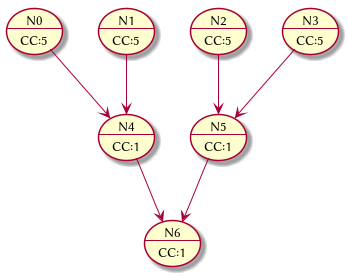
\includegraphics[width=.4\linewidth]{grafo1}
  \caption{Grafo A}
  \label{fig:grafo1}
\end{figure}

\begin{figure}[H]
  \centering
  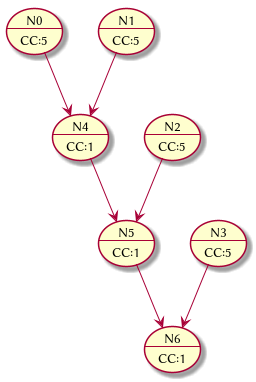
\includegraphics[width=.4\linewidth]{grafo2}
  \caption{Grafo B}
  \label{fig:grafo2}
\end{figure}

\subsection{Soluci\'on Grafo A}
\label{pnt:sgra}
\subsubsection{M\'aximo Grado de Concurrencia}
Iniciamos con el calculo del M\'aximo Grado de Concurrencia, el cual en este
caso, mediante el an\'alisis del Grafo presentado en la \texttt{Figura
\ref{fig:grafo1}} es de $4$

\subsubsection{Camino cr\'itico}
Mediante el analisis del grafo en la \texttt{Figura
\ref{fig:grafo1}} se procede a identificar el camino critico de forma sencilla
este se presenta en la \texttt{Figura \ref{fig:cc1}}
\begin{figure}[H]
  \centering
  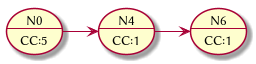
\includegraphics[width=.4\linewidth]{grafo1_cc}
  \caption{Camino cr\'itico para el grafo en la figura \ref{fig:grafo1}}
  \label{fig:cc1}
\end{figure}

\subsubsection{Grado Medio de Concurrencia}
El valor de $L=7$ en este caso sale de realizar la suma de los pesos de los
nodos que conforman el grafo en la \texttt{Figura \ref{fig:cc1}}, se procede a mostrar
el Grado Medio de Concurrencia presentado en el \texttt{Desarrollo \ref{eq1}}

\begin{equation} \label{eq1}
\begin{split}
\frac{\sum_{i=0}^{N} coste(nodo_{i})}{L} & =  \frac{5 + 5 + 5 + 5 + 1 + 1 + 1}{5 + 1 + 1} \\
 & = \frac{23}{7} \\
 & = 3,2857
\end{split}
\end{equation}

\subsection{Soluci\'on Grafo B}
\subsubsection{M\'aximo Grado de Concurrencia}
Nuevamente procedemos con el calculo del M\'aximo Grado de Concurrencia, el cual en este
caso, mediante el an\'alisis del Grafo presentado en la \texttt{Figura
\ref{fig:grafo2}} tambi\'en se determina que es de $4$

\subsubsection{Camino cr\'itico}
Mediante el an\'alisis del grafo en la \texttt{Figura
\ref{fig:grafo2}} se procede a identificar el camino cr\'itico de la misma manera
realizada en el \texttt{Punto \ref{pnt:sgra}} este se presenta en la
\texttt{Figura \ref{fig:cc2}}
\begin{figure}[H]
  \centering
  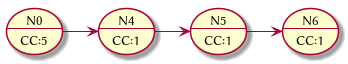
\includegraphics[width=.4\linewidth]{grafo2_cc}
  \caption{Camino cr\'itico para el grafo en la figura \ref{fig:grafo2}}
  \label{fig:cc2}
\end{figure}

\subsubsection{Grado Medio de Concurrencia}
El valor de $L=8$, se llega a la conclusi\'on en del mismo modo que para el
ejercicio desarrollado en el \texttt{Punto \ref{pnt:sgra}}. Se procede a mostrar
el Grado Medio de Concurrencia en el \texttt{Desarrollo \ref{eq2}}

\begin{equation} \label{eq2}
\begin{split}
\frac{\sum_{i=0}^{N} coste(nodo_{i})}{L} & =  \frac{5 + 5 + 5 + 5 + 1 + 1 +
1}{5 + 1 + 1 + 1} \\
 & = \frac{23}{8} \\
 & = 2,875
\end{split}
\end{equation}


\subsection{Grafo de dependencia 2}
\textsc{Consigna}: \textbf{se tiene 2 grafos de dependecias \texttt{Figura
\ref{gr:an1}} y \texttt{Figura \ref{gr:an2}} que representan 2 posibles
soluciones a una consulta sobre una base de datos. Calcule el Grado Medio de
Concurrencia de cada grafo de dependencia, siendo el peso de cada nodo igual a
la cantidad de registros que recupera.}

\begin{figure}[H]
  \centering
  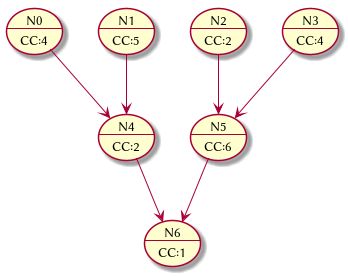
\includegraphics[width=.4\linewidth]{gr_an1}
  \caption{Grafo Dependencias: Consulta 1}
  \label{gr:an1}
\end{figure}

\begin{figure}[H]
  \centering
  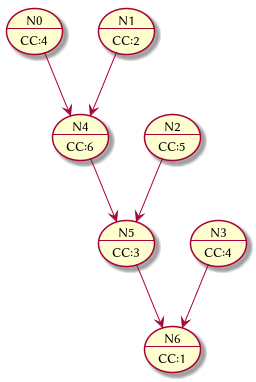
\includegraphics[width=.4\linewidth]{gr_an2}
  \caption{Grafo Dependencias: Consulta 2}
  \label{gr:an2}
\end{figure}

\subsection{Soluci\'on Consulta 1}
\subsubsection{Camino cr\'itico}
Mediante el analisis del grafo en la \texttt{Figura \ref{gr:an1}} se procede
a identificar el camino cr\'itico de la misma manera realizada en los puntos anteriores,
el grafo correspondiente se presenta en la \texttt{Figura \ref{fig:an1_cc}}
\begin{figure}[H]
  \centering
  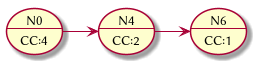
\includegraphics[width=.4\linewidth]{gr_an1_cc}
  \caption{Camino cr\'itico para el grafo en la figura \ref{gr:an1}}
  \label{fig:an1_cc}
\end{figure}

\subsubsection{Grado Medio de Concurrencia}
El valor de $L=7$, se llega a la conclusi\'on en del mismo modo que para el
ejercicio desarrollado en el \texttt{Punto \ref{pnt:sgra}}, esto es, sumando
los pesos de los nodos que conforman
el grafo en la \texttt{figura \ref{fig:cc2}}, se procede a mostrar
el Grado Medio de Concurrencia presentado en el \texttt{Desarrollo \ref{eq3}}

\begin{equation} \label{eq3}
\begin{split}
\frac{\sum_{i=0}^{N} coste(nodo_{i})}{L} & =  \frac{4 + 5 + 2 + 4 + 2 + 6 + 1}{4 + 2 + 1} \\
 & = \frac{24}{7} \\
 & = 3,4285
\end{split}
\end{equation}

\subsection{Soluci\'on Consulta 2}
\subsubsection{Camino cr\'itico}
Mediante el analisis del grafo en la \texttt{Figura
\ref{gr:an2}} se procede a identificar el camino cr\'itico de la misma manera
realizada en los puntos anteriores, el grafo correspondiente se presenta en la
\texttt{Figura \ref{fig:an2_cc}}
\begin{figure}[H]
  \centering
  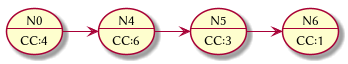
\includegraphics[width=.4\linewidth]{gr_an2_cc}
  \caption{Camino cr\'itico para el grafo en la figura \ref{gr:an2}}
  \label{fig:an2_cc}
\end{figure}

\subsubsection{Grado Medio de Concurrencia}
El valor de $L=14$, se llega a la conclusi\'on en del mismo modo que para el
ejercicio desarrollado en el \texttt{Punto \ref{pnt:sgra}}, esto es, sumando
los pesos de los nodos que conforman el grafo en la \texttt{figura
\ref{fig:an2_cc}},
se procede a mostrar el Grado Medio de Concurrencia presentado en el
\texttt{Desarrollo \ref{eq4}}

\begin{equation} \label{eq4}
\begin{split}
\frac{\sum_{i=0}^{N} coste(nodo_{i})}{L} & =  \frac{4 + 2 + 5 + 4 + 6 + 3 +
1}{4 + 6 + 3 + 1} \\
 & = \frac{24}{14} \\
 & = 1,7142
\end{split}
\end{equation}


\section{Descomposici\'on}
\textsc{Consigna}: \textbf{?`Cu\'al es el objetivo principal de la
descomposici\'on? Describa brevemente los tipos de descomposic\'on.}\\

El objetivo principal de la descomposici\'on es \textit{lograr un buen uso de
los recusos disponibles} por parte de la aplicaci\'on, minimizando el tiempo en
el que se realicen operaciones. Los tipos de descomposici\'on se describen a
continuaci\'on:

\begin{itemize}
\item Generales
	\begin{itemize}
	\item \textbf{Descomposici\'on de dominio}: es la divisi\'on de un
programa en sub-divisiones que indican cuales son las funciones que deben
contemplar. Es aconsejable utilizarlo cuando la estructura de datos es la m\'as
utilizada o la m\'as grande.
	\item \textbf{Descomposici\'on funcional}: es la divisi\'on de las
funciones de un programa, siendo procesadas de manera concurrente. Esta
t\'ecnica puede ser utilizada siempre y cuando no ocasione excesiva
comunicaci\'on y/o solapamiento en los datos.
	\item \textbf{Descomposici\'on recursiva}: bas\'andose en una t\'ecnica
secuencial divide las funciones de un programa en forma recursiva y
combinaci\'on de resultados.
	\end{itemize}
\item Espec\'ificos
	\begin{itemize}
	\item \textbf{Descomposici\'on exploratoria}: se utilizan en problemas
de b\'usqueda, se divide el espacio de b\'usqueda en partes m\'as peque\~nas.
	\end{itemize}
\item Mixtos
	\begin{itemize}
	\item Una combinaci\'on de los anteriores.
	\end{itemize}
\end{itemize}

\section{Asignaci\'on, ?`Qu\'e funci\'on cumple?}
La funci\'on que cumple, es la de asignar las tareas a cada procesador,
minimizando el costo en las comunicaciones y maximizando la utilizaci\'on de los
procesadores involucrados.

\section{Ociosidad}
\textsc{Consigna}: \textbf{?`Qu\'e es la ociosidad? ?`Cu\'ales son sus principales motivos?}
\subsection{?`Qu\'e es la ociosidad?}
El t\'ermino est\'a asociado al tiempo libre que iene un procesador esperando
por realizar alguna tarea.

\subsection{?`Cu\'ales son sus principales motivos?}
Entre los principales motivos para la ociosidad se encuentran:
\begin{itemize}
\item \textbf{Desequilibrio de carga}: se busca equilibrar tanto los
c\'alculos como las comunicaciones.
\item \textbf{Espera entre procesos}: esto se da cuando existe una alta
interdependencia entre los procesos encargados de realizar una tarea.
\end{itemize}

\section{Estrat\'egias de Asignaci\'on}
\textsc{Consigna}: \textbf{describa brevemente las estrategias generales de
asignaci\'on.}\\

Las estrategias generales de asignaci\'on se describen a continuaci\'on:
\begin{itemize}
\item Agrupamiento:
	\begin{itemize}
	\item Buscan agrupar un conjunto de tareas para mejorar la localidad.
	\item Minimizar el volumen de datos.
	Esto se puede lograr mediante lo siguiente:
		\begin{itemize}
		\item Agrupamiento por bloques de elementos continuos
		\item Agrupar tareas que se comuniquen mucho.
		\item El uso de datos locales para almacenar resultados
intermedios.
		\end{itemize}
	\item Reducci\'on de la frecuencia de interacciones.
	Esto se logra mediante lo siguiente:
		\begin{itemize}
		\item Memoria comartida: algoritmos por bloques reduce
p\'erdidas de cach\'e.
		\item Memoria distribuida: agrupar mensajes.
		\end{itemize}
	\end{itemize}
\item Replicaci\'on:
	\begin{itemize}
	\item
	\end{itemize}
\end{itemize}

\section{Grafo de Precedencias}
\textsc{Consigna}: \textbf{Dado el fragmento de programa concurrente en el \texttt{Listing \ref{graprec}} obtener el grafo de precedencia asociado}.
\newpage
\begin{lstlisting}[caption={Fragmento de programa concurrente}, label=graprec]
P0;
COBEGIN
	P1;
	P2;
	COBEGIN
		P3; P4; P5; P6;
	COEND
	P7;
COEND
P8;
\end{lstlisting}

A continuaci\'on se presenta el grafo de precedencia, la justificaci\'on del
\textit{por qu\'e} se realiz\'o de esa manera, espec\'ificamente, la parte del
\texttt{Gr\'afico \ref{fig:graprec}} que se encuenra encerrado en un
rect\'angulo; lo que se hizo tiene sus bases en dos cuestiones mencionadas
en el cursado de la materia.
\begin{itemize}
\item La primera de ellas tiene que ver con lo mencionado en
\cite{gortazarbellas}, y expuesto adem\'as en una de las diapositivas de la
c\'atedra y tiene que ver con el orden en el cual ocurre la ejecuci\'on de los
diferentes procesos que se quiere paralelizar, en resumen, este
acontecimiento es aleatorio, se elige un proceso al azar para ser ejecutado.
\item la otra parte, se expuso en clases durante la explicaci\'on de
\textbf{qu\'e es un grafo de dependencias}, en donde se dejo constancia de que
para que se pueda iniciar una tarea, debe ejecutarse, en primer lugar, la tarea fuente.
\end{itemize}


\begin{figure}[H]
  \centering
  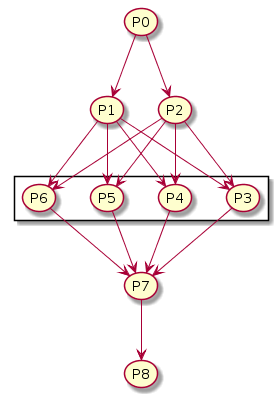
\includegraphics[width=.4\linewidth]{grafo_precedencia.png}
  \caption{Grafo de precedencia para \texttt{Listing \ref{graprec}}}
  \label{fig:graprec}
\end{figure}

En este caso tenemos a P1 y P2 como tareas fuente, las cuales deben finalizar,
de ah\'i se determina cual es la tarea siguiente, por lo expuesto en el primero
de los dos puntos que se mencionaron anteriormente, la selecci\'on ser\'a al azar,
por tanto, se consideran todos los posibles escenarios de finalizaci\'on de los padres.

% === Bibliografia === %
\newpage
\begin{thebibliography}{99}
	% Item 1
	\bibitem[Gort\'azar Bellas, et al, 2012]{gortazarbellas}\textsc{Gort\'azar Bellas, Francisco; Mart\'inez Unanue, Raquel; Fresno Fern\'andez, Victor}. \textit{Lenguajes de Programaci\'on y Procesadores - Cap\'itulo 3.5}. Editorial Universitaria Ramon Areces, Madrid, 2012. \textsc{ISBN: 9788499610702}.
\end{thebibliography}
\end{document}
